  The real results
  \begin{figure}[ht]
      \centering
      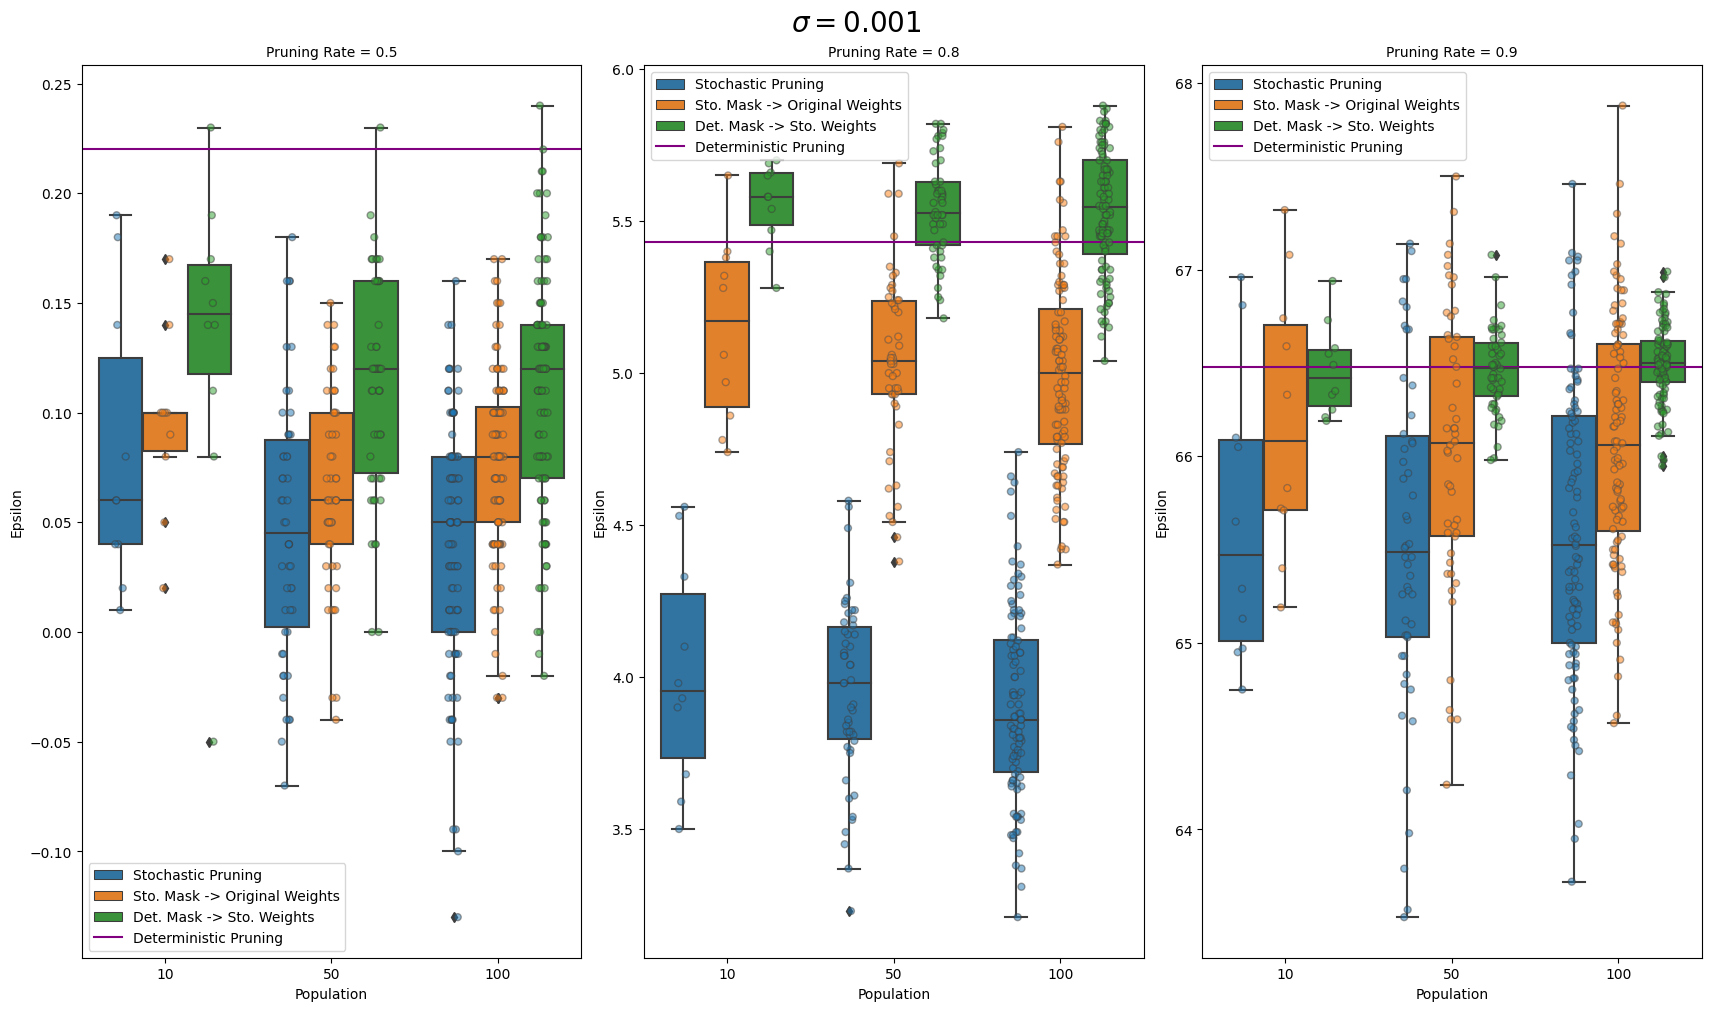
\includegraphics[width=\columnwidth]
      {epsilon_allN_all_pr_sigma=0.001.png}
      \caption{Epsilon for $\sigma=0.001$ varying population size and different
      pruning rates}
      \label{fig:allNS0.001}
  \end{figure}
  \begin{figure}[ht]
      \centering
      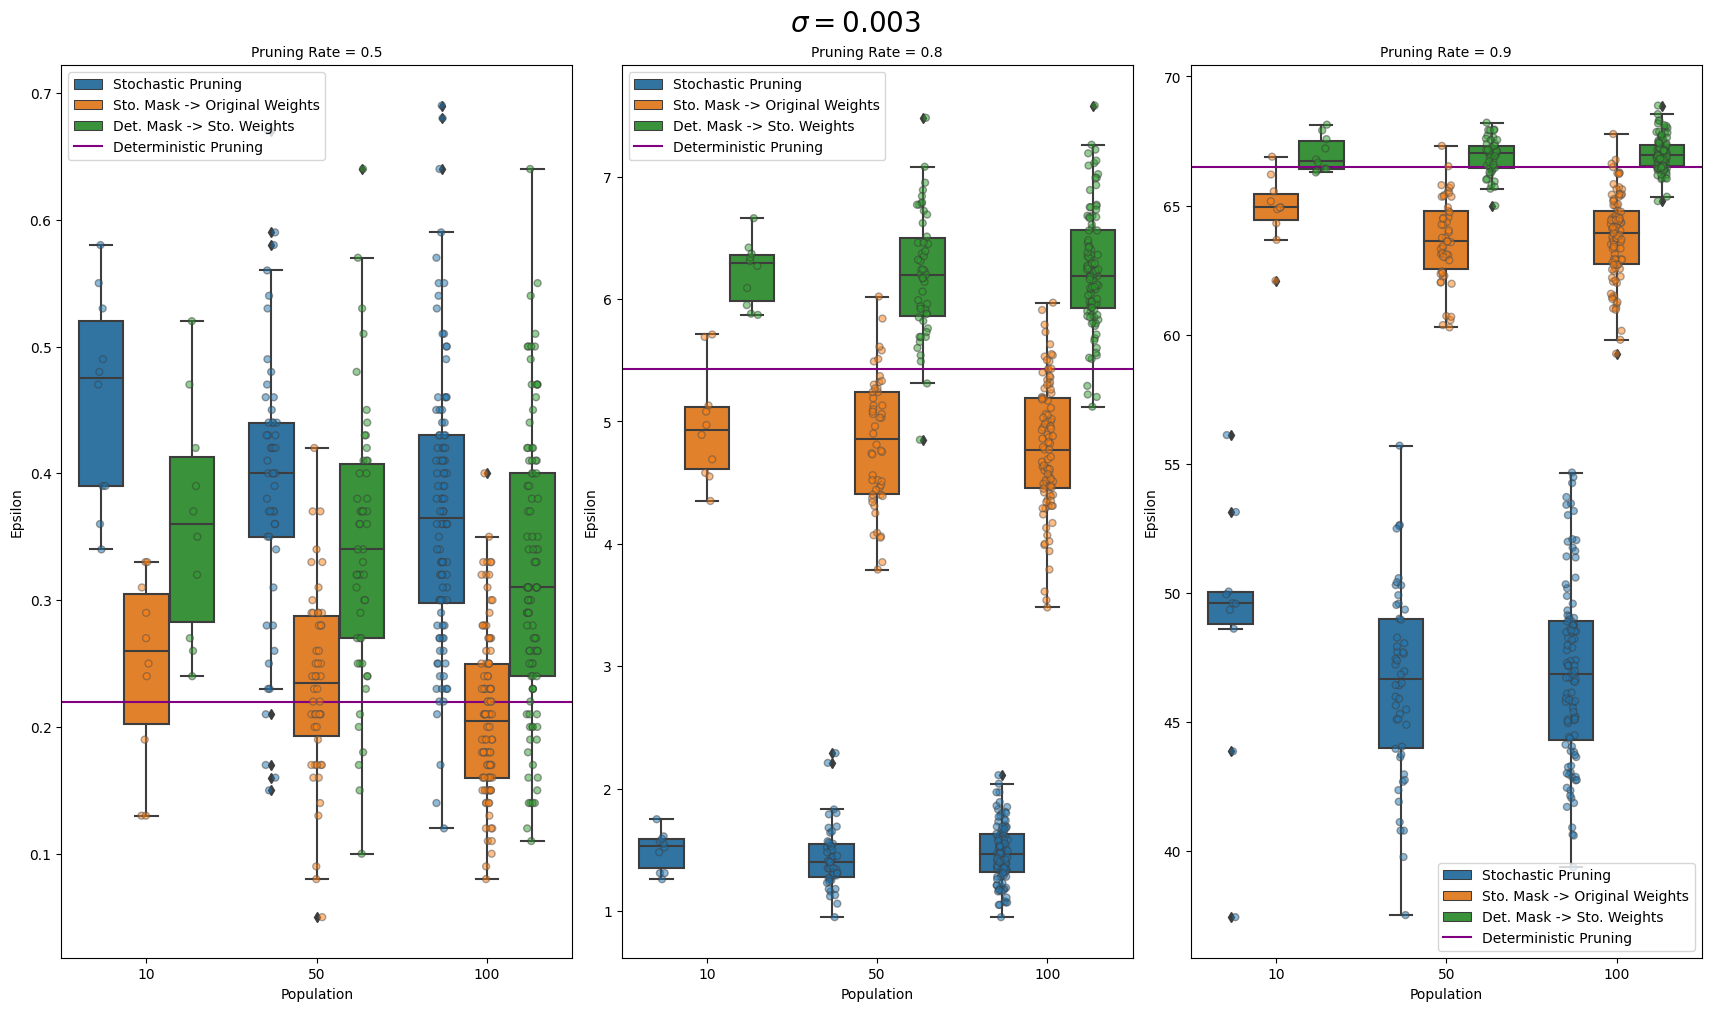
\includegraphics[width=\columnwidth]
      {epsilon_allN_all_pr_sigma=0.003.png}
      \caption{Epsilon for $\sigma=0.003$ varying population size and different
      pruning rates}
      \label{fig:allNS0.003}
  \end{figure}
  \begin{figure}[ht]
      \centering
      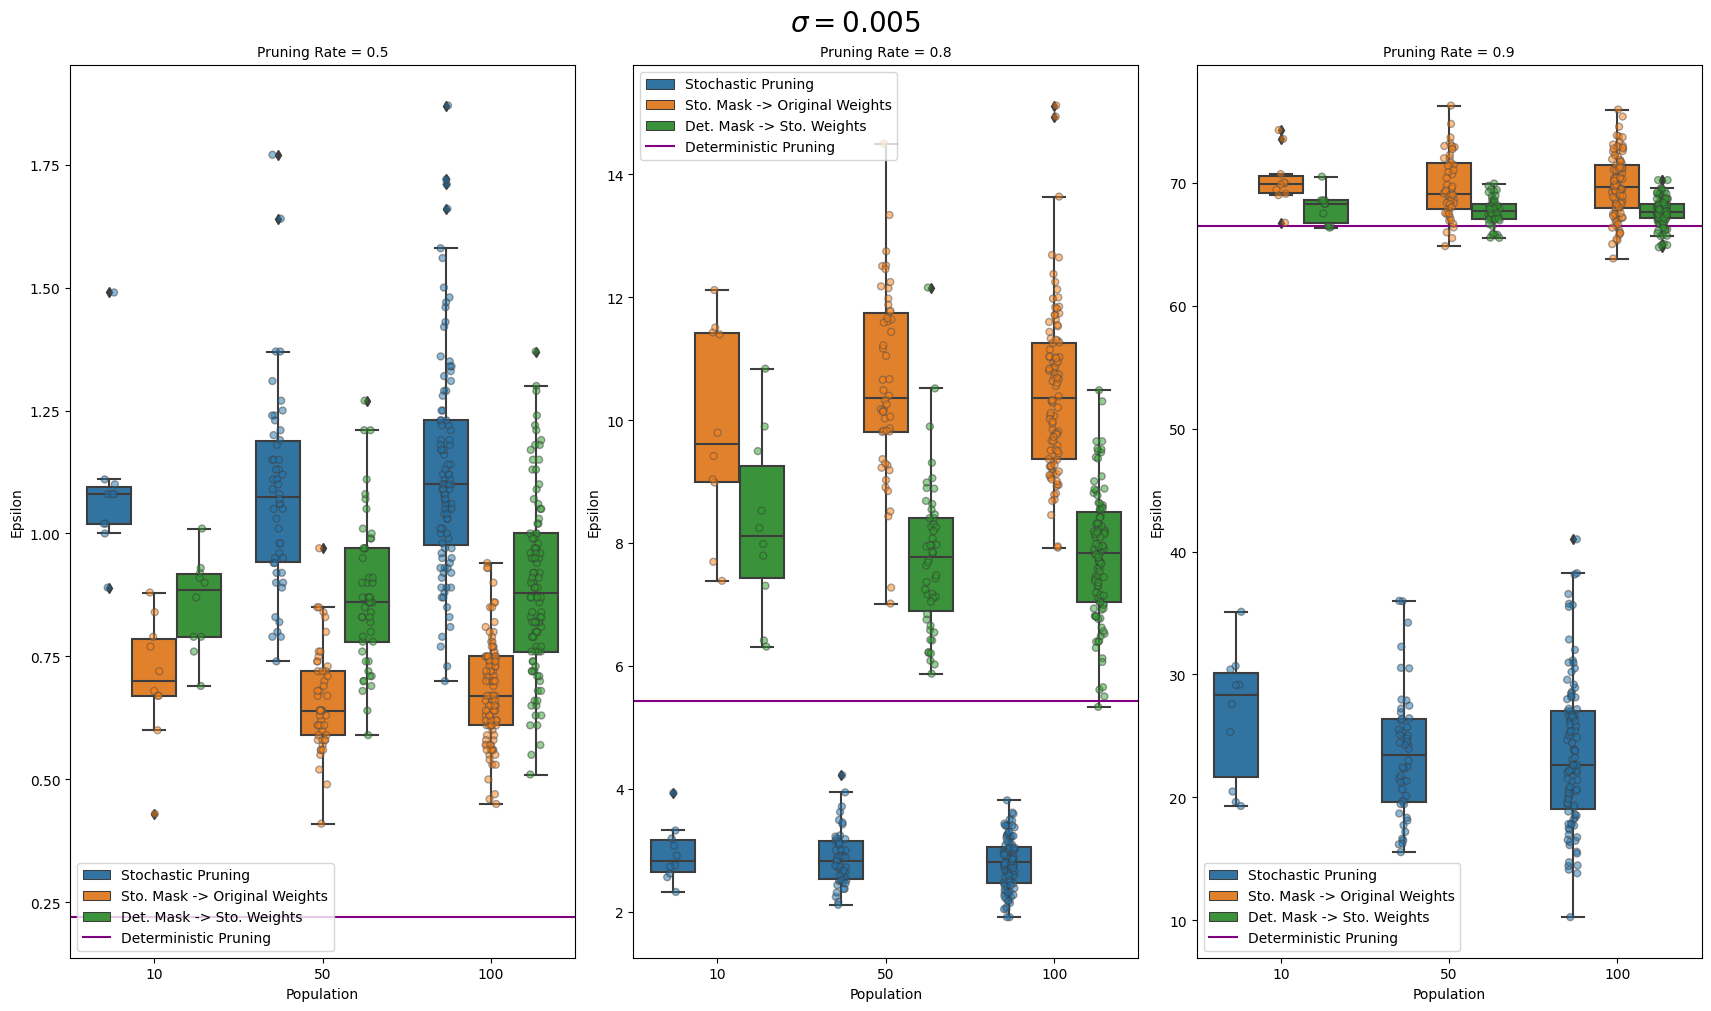
\includegraphics[width=\columnwidth]
      {epsilon_allN_all_pr_sigma=0.005.png}
      \caption{Epsilon for $\sigma=0.005$ varying population size and different
      pruning rates}
      \label{fig:allNS0.005}
  \end{figure}
